\documentclass[11pt]{article}

\usepackage{amsmath}
\usepackage{amssymb}
\usepackage{array}
\usepackage{geometry}
\usepackage{enumitem}
\usepackage{float}
\usepackage{cancel}
\usepackage{graphicx}
\usepackage[labelformat=empty]{caption}
\usepackage{booktabs}

\geometry{
	a4paper,
 	left=20mm,
 	top=20mm,
 	bottom=20mm,
}

\setlength{\parindent}{0pt}

\begin{document}

\section{Mengen}

\subsection{Definitionen}

\begin{description}[labelindent=16pt,style=multiline,leftmargin=6cm, noitemsep]
	\item[Obere/Untere Schranke:] $\exists b \in \mathbb{R}\ \forall a\in A:\ a \leq b$, $\exists c \in \mathbb{R}\ \forall a\in A:\ a \geq c$
	\item[Supremum:] kleinste obere Schranke $\sup A$
	\item[Infimum:] gr{\"o}sste untere Schranke $\inf A$
	\item[Maximum/Minimum:] $\sup A \in A$, $\inf A \in A$
	\item[kompakt:] abgeschlossen und beschr{\"a}nkt
	\item[abgeschlossen:] z.B. $[0,1]$
\end{description}

\subsubsection{Vorgehen zur Bestimmung von Maximum/Minimum}

\begin{enumerate}[noitemsep]
	\item Zeigen, dass $f(x)$ stetig ist
	\item Zeigen, dass Definitionsmenge kompakt ist
	\item Nach \textbf{Satz von Weierstrass} wird Maximum/Minimum angenommen
	\item Maximum/Minimum bestimmen
\end{enumerate}

\subsection{Identit{\"a}ten}

\begin{equation*}
\begin{split}
	A + B & := \{a + b | a \in A, b \in B\} \\
	\sup(A+B) = \sup A + \sup B,\ & \inf(A+B) = \inf A + \inf B \\
	\sup(A \cup B) = \max\{\sup A, \sup B\},\ & \inf(A \cup B) = \min\{\inf A, \inf B\}
\end{split}
\end{equation*}

\section{Komplexe Zahlen}

\begin{minipage}[c]{0.5\textwidth}
\centering
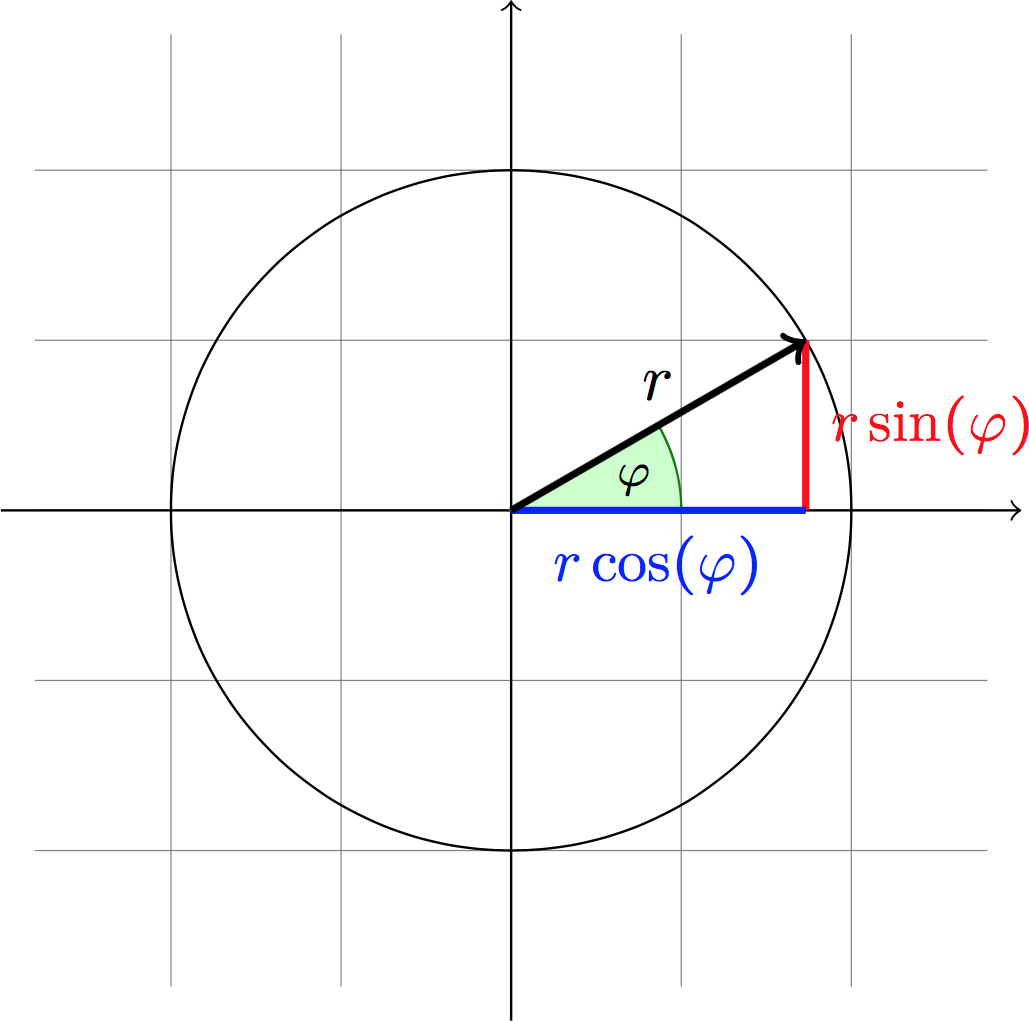
\includegraphics[width=\linewidth,keepaspectratio=true]{images/polarform}
\end{minipage}
%
\begin{minipage}[c]{0.5\textwidth}
\begin{equation*}
\begin{split}
	z & = x + iy = r(\cos(\varphi) + i\sin(\varphi)) = re^{i\varphi} \\
	r & = |z| = \sqrt{x^2 + y^2} \\
	\arg(z) & = \varphi  = \arctan(\frac{y}{x}) \quad \text{(je nach Quadrant)}  \\
	x & = r\cos(\varphi) \\
	y & = r\sin(\varphi) \\
	zw & = (re^{i\varphi})\cdot(se^{i\psi}) = rse^{i(\varphi + \psi)} \\
	\sqrt[q]{z} & = \sqrt[q]{s}e^{i\phi}\text{, wobei }\phi = \frac{\varphi}{q} \mod \frac{2\pi}{q} \\
	e^{i(\frac{\pi}{2} + 2\pi k)} & = i,\ e^{i\pi} = 1, \ e^{-i\pi} = -1
\end{split}
\end{equation*}
\end{minipage}

\begin{minipage}[c]{0.5\textwidth}
\begin{equation*}
\begin{split}
	(a,b) \cdot (c, d) & = (ac-bd, ad+bc) \\
	\overline{z} & = x - iy\\
	z^{-1} & = \frac{\overline{z}}{|z|^2} \\
	i & = \sqrt{-1}\\
\end{split}
\end{equation*}
\end{minipage}
%
\begin{minipage}[c]{0.5\textwidth}
\begin{equation*}
\begin{split}
	i^2 & = -1 \\
	|z|^2 & = z\overline{z} \\
	|zw|^2 & = (zw) \cdot \overline{(zw)} = |z|^2|w|^2
\end{split}
\end{equation*}
\end{minipage}

\section{Grenzwert}

\subsection{Dominanz}

\begin{equation*}
\begin{split}
	\text{F{\"u}r}\ x \to +\infty:\quad & ... < \log(\log(x)) < \log(x) < x^\alpha < \alpha^x < x! < x^x \\
	\text{F{\"u}r}\ x \to 0:\quad & ... < \log(\log(x)) < \log(x) < (\frac{1}{x})^\alpha \\
\end{split}
\end{equation*}

\subsection{Fundamentallimes}

\begin{equation*}
\begin{split}
	\lim_{x \to a} \frac{\sin \odot}{\odot} = \lim_{x \to a} \frac{\tan \odot}{\odot} & = 1\ \text{mit}\ \odot \xrightarrow{\: x \to a \: } 0 \\ 
	\lim_{x \to a} (1 + \frac{1}{\odot})^\odot & = e\ \text{mit}\ \odot \xrightarrow{\: x \to a \: } \infty \\ 
	\lim_{x \to a} (1 + \odot)^\frac{1}{\odot} & = e\ \text{mit}\ \odot \xrightarrow{\: x \to a \: } 0 \\ 
\end{split}
\end{equation*}

\subsection{Wurzeltrick}

\begin{equation*}
	\lim_{x\to\infty} \sqrt{\alpha}+\beta = \lim_{x\to\infty}(\sqrt{\alpha}+\beta)\frac{\sqrt{\alpha}-\beta}{\sqrt{\alpha}-\beta}
\end{equation*}

\subsection{$e^{\log(x)}$-Trick}

\paragraph{Anforderung:}Term der Form $f(x)^{g(x)}$ mit Grenzwert "$0^0$", "$\infty^0$" oder "$1^\infty$" f{\"u}r $x \to 0$

\begin{equation*}
	\textbf{Grundsatz:}\quad\lim_{x\to a}f(x)^{g(x)} = \lim_{x\to a}e^{g(x) \cdot \log(f(x))}
\end{equation*}

\emph{Tipp:} Danach den Limes des Exponenten berechnen. Oft ist Bernoulli-de l'H{\^o}pital dazu n{\"u}tzlich.

\subsection{Substitution}

\begin{equation*}
\begin{split}
	\lim_{x\to \infty} x^2(1 - \cos(\frac{1}{x})) \Rightarrow u = \frac{1}{x} \Rightarrow \lim_{x\to 0} \frac{1 - \cos(u)}{u^2}
\end{split}
\end{equation*}

\subsection{Satz von Bernoulli-de l'H{\^o}pital}

\paragraph{Anforderung:}Term der Form $\frac{f(x)}{g(x)}$ mit Grenzwert entweder "$\frac{0}{0}$" oder "$\frac{\infty}{\infty}$" mit $g'(x) \neq 0$. \\

\begin{equation*}
	\textbf{Grundsatz:}\quad\lim_{x\to a}\frac{f(x)}{g(x)} = \lim_{x\to a}\frac{f'(x)}{g'(x)}
\end{equation*}

\begin{table}[H]
\centering
\begin{tabular}{|c|c|c|}
\hline
\textbf{Term} & \textbf{Anforderung} & \textbf{Umformung} \\ \hline
$f(x)g(x)$              & "$0\cdot\infty$"                     & $\frac{g(x)}{\frac{1}{f(x)}}$          \\ \hline 
$\frac{f(x)}{g(x)} - \frac{h(x)}{i(x)}$ & "$\infty - \infty$"  & $\frac{f(x)i(x) - h(x)g(x)}{g(x)i(x)}$ \\ \hline      
\end{tabular}
\end{table}

\subsection{Wichtige Grenzwerte}

\begin{equation*}
\begin{split}
	\lim\limits_{n \to \infty} \left( 1+\frac{x}{n} \right)^n = e^x \qquad & \qquad \lim\limits_{n \to \infty} \left( 1+\frac{1}{n} \right)^n = e \\
	\lim\limits_{x \to 0} \frac{a^x-1}{x} = \ln a \qquad & \qquad \lim\limits_{x \to 0} \frac{\log_a(1+x)}{x} = \frac{1}{\ln a} \\
	\lim\limits_{x \to 0} \frac{1-\cos(x)}{x} = 0 \quad \qquad & \qquad \lim\limits_{x \to 0} \frac{1-\cos(x)}{x^2} = \frac{1}{2} \\
	\lim\limits_{x \to 0} \frac{\tan(x)}{x} = 1 \qquad & \qquad \lim\limits_{x \to 0} \frac{\sin(x)}{x} = 1 \\
	\lim\limits_{n \to \infty} \frac{n!}{n^n} = 0 \qquad & \qquad \lim\limits_{n \to 0} \frac{e^n -1 }{n} = 1 \\
	\lim\limits_{n \to \infty} \sqrt[n]{n!} = \infty \qquad & \qquad \lim\limits_{n \to \infty} \sqrt[n]{n} = 1 \\
	\lim\limits_{n \to \infty} \ln(n) = \infty \qquad & \qquad \lim\limits_{x \to 0} \frac{\log_a(1+x)}{x} = \frac{1}{\ln a} \\
\end{split}
\end{equation*}

\section{Folgen}

\subsection{Definition}

\begin{equation*}
\begin{split}
	\textbf{Konvergenz:} \quad & \forall \varepsilon > 0\ \exists N = N(\varepsilon) \in \mathbb{N},\ \text{sodass}\ \forall n \geq N: |a_n - a| < \varepsilon \\
	\textbf{Divergenz:} \quad & \forall K > 0\ \exists N = N(K) \in \mathbb{N},\ \text{sodass}\ \forall n \geq N: |a_n| > K
\end{split}
\end{equation*}

\subsection{Beweis}

\begin{enumerate}[noitemsep]
	\item Zeige mittels \textbf{Induktion}, dass die Folge \textbf{beschr{\"a}nkt} ist und monoton \textbf{steigt/f{\"a}llt}. Benutze dazu z.B. folgende Aussagen: $a_n \leq a_{n+1}$ oder $a_{n+1}-a_n \geq 0$.
	\item \textbf{Grenzwert berechnen} mit $a := \lim_{n \to \infty} a_n$ oder durch die ersten paar Terme absch{\"a}tzen
	\item Beweise den Grenzwert (z.B. mit $a_n \geq a$) um Beschr{\"a}nktheit zu beweisen
\end{enumerate}

\emph{Tipp:} Den Grenzwert in der rekursiven Formel mit $a_n$ und $a_{n+1}$ ersetzen. \\
F{\"u}r die Formel $a_{n+1} = \frac{1}{2}a_n + \sqrt{a_n}$ muss zum Beispiel gelten: $a = \frac{1}{2}a + \sqrt{a}$ (hier $a = 4$)

\section{Reihen $\sum^\infty$}

\subsection{Konvergenzkriterien}

\begin{table}[H]
\centering
\begin{tabular}{|p{5cm}|p{4cm}|p{5cm}|}
\hline
                                             & \textbf{Eignung}    & \textbf{Bemerkung}                        \\ \hline
\textbf{Limes des allgemeinen Glieds}        &                     & zeigt nur Divergenz                       \\ \hline
\textbf{Majoranten- und Minorantenkriterium} &                     & ersten Glieder spielen keine Rolle        \\ \hline
\textbf{Quotientenkriterium}                 & $a_n$ mit Faktoren wie $n!$, $a^n$, oder Polynome & gleiche Folgerung wie Wurzelkriterium     \\ \hline
\textbf{Wurzelkriterium}                     & $a_n = (b_n)^n$     & gleiche Folgerung wie Quotientenkriterium \\ \hline
\textbf{Leibnitz-Kriterium}                  & $\sin$, $\cos$, $\tan$, $(-1)^n$ &                                           \\ \hline
\textbf{Absolute Konvergenz}                 & $\sin$, $\cos$, $\tan$, $(-1)^n$   &                                           \\ \hline
\textbf{Sandwich-Theorem}					 & $\sin$, $\cos$, $\tan$, $(-1)^n$ & \\ \hline
\end{tabular}
\end{table}

\clearpage

\subsubsection*{Limes des allgemeinen Glieds}

\paragraph{Bemerkung:} Mit dieser Methode l{\"a}sst sich nur die Divergenz beweisen, nicht jedoch die Konvergenz.

\begin{enumerate}
	\item $\sum_n a_n$ gegeben
	\item Grenzwert $\lim_{n\mapsto\infty} a_n$ berechnen
	\begin{itemize}
		\item falls Grenzwert $\neq 0 \Rightarrow$ \textbf{divergent} 
		\item falls Grenzwert $= 0 \Rightarrow$ keine Aussage 
	\end{itemize}
\end{enumerate}

\subsubsection*{Majoranten- und Minorantenkriterium}

Es seien $a_n$, $b_n > 0$ mit $a_n \geq b_n\ \forall n$ ab einem gewissen $n_0$. Dann gilt: 
\begin{equation*}
\begin{split}
	\sum_n a_n \text{ konvergent} & \Rightarrow \sum_n b_n \textbf{ konvergent}\quad \text{(Majorantenkriterium)} \\
	\sum_n b_n \text{ divergent} & \Rightarrow \sum_n a_n \textbf{ divergent}\quad \text{(Minorantenkriterium)} \\
\end{split}
\end{equation*}

\subsubsection*{Vergleichskriterium}

\begin{enumerate}
	\item $\sum_n a_n$ und $\sum_n b_n$ gegeben mit $a_n,b_n > 0$
	\item Grenzwert $\lim_{n\mapsto\infty} \frac{a_n}{b_n}$ berechnen
	\begin{itemize}
		\item falls Grenzwert $= 0$:
		\begin{itemize}
			\item $\sum_n a_n$ divergent $\Rightarrow \sum_n b_n$ \textbf{divergent}
			\item $\sum_n b_n$ konvergent $\Rightarrow \sum_n a_n$ \textbf{konvergent}
		\end{itemize} 
		\item falls Grenzwert $= \infty$:
		\begin{itemize}
			\item $\sum_n a_n$ konvergent $\Rightarrow \sum_n b_n$ \textbf{konvergent}
			\item $\sum_n b_n$ divergent $\Rightarrow \sum_n a_n$ \textbf{divergent}
		\end{itemize} 
	\end{itemize}
\end{enumerate}

\subsubsection*{Quotientenkriterium}

\begin{enumerate}
	\item $\sum_n a_n$ mit $a_n \neq 0$ gegeben
	\item Grenzwert $\lim_{n\mapsto\infty}|\frac{a_{n+1}}{a_n}|$ berechnen
	\begin{itemize}
		\item falls Grenzwert $> 1 \Rightarrow$ \textbf{divergent}
		\item falls Grenzwert $< 1 \Rightarrow$ \textbf{konvergent}
		\item falls Grenzwert $= 1 \Rightarrow$ keine Aussage
	\end{itemize}
\end{enumerate}

\subsubsection*{Wurzelkriterium}

\begin{enumerate}
	\item $\sum_n a_n$ mit $a_n \neq 0$ gegeben
	\item Grenzwert $\lim_{n\mapsto\infty}\sqrt[n]{|a_n|}$ berechnen
	\begin{itemize}
		\item falls Grenzwert $> 1 \Rightarrow$ \textbf{divergent}
		\item falls Grenzwert $< 1 \Rightarrow$ \textbf{konvergent}
		\item falls Grenzwert $= 1 \Rightarrow$ keine Aussage
	\end{itemize}
\end{enumerate}

\subsubsection*{Leibniz-Kriterium}

\begin{enumerate}
	\item $\sum_n (-1)^n a_n$ gegeben
	\item \textbf{konvergent}, falls:
	\begin{enumerate}
		\item $a_n \geq 0$
		\item $\lim_{n\mapsto\infty} a_n = 0$
		\item $a_n$ monoton fallend
	\end{enumerate}
\end{enumerate}

\subsubsection*{Absolute Konvergenz}

\begin{enumerate}
	\item $\sum_n (-1)^n a_n$ gegeben
	\item \textbf{konvergent}, falls $\sum_n |a_n|$ konvergent
\end{enumerate}

\subsection{Geometrische Reihe}

Reihe der Form $\sum^\infty_{k = 0} a \cdot r^k$ mit der \textbf{Partialsumme}:

\begin{equation*}
	S_N=\frac{a-ar^{N+1}}{1-r}
\end{equation*}

\textbf{Konvergent}, falls $0<|r|<1$ mit Grenzwert:

\begin{equation*}
	\sum^\infty_{k=0}ar^k=\frac{a}{1-r}
\end{equation*}

\subsection{Potenzreihe}

Reihe der Form $\sum^\infty_0 a_nx^n$. \textbf{Konvergent}, falls $|x|<\rho$. In diesem Gebiet darf man die Reihe ableiten und integrieren.

\begin{equation*}
	\rho= \lim_{n\rightarrow \infty}|\frac{a_n}{a_{n+1}}|
\end{equation*}
\begin{equation*}
	\rho=\frac{1}{\lim_{n\rightarrow \infty}\sqrt[n]{|a_n|}}
\end{equation*}

\paragraph{Konvergenzverhalten am Rand:} Es muss noch {\"u}berpr{\"u}ft werden, ob die Reihe f{\"u}r genau $\rho$ konvergiert. Dazu muss $\rho$ in die Formel eingesetzt werden.

\subsubsection{Wichtige Reihen}

\begin{minipage}[c]{0.5\textwidth}
\begin{equation*}
\begin{split}
	\cos(x) & = \sum^\infty_{n =0}\frac{(-1)^nx^{2n}}{(2n)!} \\
	\sin(x) & = \sum^\infty_{n =0}\frac{(-1)^nx^{2n+1}}{(2n+1)!} \\
	e^x & = \sum^\infty_{n =0}\frac{x^n}{n!} \\
\end{split}
\end{equation*}

\end{minipage}
%
\begin{minipage}[c]{0.5\textwidth}
\begin{equation*}
\begin{split}
	n^2 & = \sum_{k=1}^n 2k-1\\
	\sum_{n=1}^{\infty}\frac{1}{n} & = \infty\quad\text{(harmonisch)}
\end{split}
\end{equation*}
\end{minipage}

\subsubsection{Potenzreihenentwicklung}

\begin{equation*}
	\textbf{Grundsatz:} \quad f(x) = \sum_{n=0}^\infty \frac{f^{(n)}(0)}{n!} \cdot x^n
\end{equation*}

\section{Stetigkeit}

\subsection{Lipschitz-Stetigkeit}
Es existiert eine Konstante $L\in \mathbb{R}$, sodass:
\begin{equation*}
	|f(x)-f(y)|\leq L|x-y| \quad \forall x,y \in \Omega
\end{equation*}

\emph{Bemerkung:} Ist $f'$ \textbf{auf $\Omega$ beschr{\"a}nkt}, so ist $f$ Lipschitz-stetig. Lipschitz-Stetigkeit impliziert gleichm{\"a}ssige Stetigkeit.

\subsection{Weierstrass-Kriterium}
F{\"u}r alle $\epsilon > 0$ gibt es ein $\delta(\epsilon, a) >0$, sodass f{\"u}r alle $|x-a|<\delta$ gilt:
\begin{equation*}
	|f(x) -f(a)|<\epsilon
\end{equation*}

\subsection{Gleichm{\"a}ssige Stetigkeit}
F{\"u}r alle $\epsilon > 0$ gibt es ein $\delta(\epsilon) >0$, sodass f{\"u}r alle $|x-y|<\delta$ gilt:
\begin{equation*}
	|f(x)-f(y)| < \epsilon
\end{equation*}
\emph{Bemerkung:} Ist $f$ \textbf{stetig und kompakt}, dann ist sie auch gleichm{\"a}ssig stetig.

\subsection{Punktweise Konvergenz}

$f_n(x)$ konvergiert punktweise falls:
\begin{equation*}
	\forall x\in \Omega \quad \lim_{n\rightarrow\infty}f_n(x) = f(x)
\end{equation*}

\subsection{Gleichm{\"a}ssige Konvergenz}

\paragraph{Grundsatz:} Falls eine Folge stetiger Funktionen $f_n$ gleichm{\"a}ssig gegen $f$ konvergiert, muss $f$ stetig sein.\\

$f_n(x)$ konvergiert gleichm{\"a}ssig falls:
\begin{equation*}
	\lim_{n\rightarrow\infty} \sup|f_n(x) - f(x)| = 0
\end{equation*}

\emph{Bemerkung:} Gleichm{\"a}ssige Konvergenz impliziert punktweise Konvergenz.\\
\underline{Rezpet f{\"u}r gleichm{\"a}ssige Konvergenz} 
\begin{enumerate}[label=(\roman*)]
	\item Punktweiser Limes berechnen
				\[
						\lim_{n\rightarrow\infty}f_n(x) = f(x) \text{\quad = Grenzfunktion}
				\]
	\item Supremum bestimmen \\
				(Ableitung von $f_n(x)$  oder Absch{\"a}tzung benutzen)
				\[
						\sup|f_n(x) - f(x)|
				\]
	\item Limes $n \to \infty$ bestimmen (vgl. Kriterium glm. Konvergenz)
				\[
						\lim_{n\rightarrow\infty} \sup|f_n(x) - f(x)|
				\]
				Limes = 0 $\rightarrow$ Glm. konvergent mit Grenzfunktion f(x)
	\item Indirekte Methode \\
				\begin{itemize}
					\item $f(x)$ unstetig  auf $\Omega \Rightarrow$ keine glm. Konvergenz	
					\item $f(x)$ stetig, $f_n(x) \leq f_{n+1}(x) \forall x \in \Omega $ und $\Omega$ kompakt $\Rightarrow$ Glm. Konvergenz
				\end{itemize}

\end{enumerate}

\begin{equation*}
\begin{split}
	\text{gegeben:} \quad & f_n:[0,1] \mapsto \mathbb{R},\ f_n(x) = (1 - x^2)x^n \\
	\textbf{punktweisen Limes berechnen:} \quad & \lim_{n \to \infty} (1 - x^2)x^n = 0 \equiv f(x) \\
	& \Rightarrow\ \text{konvergiert gegen 0} \\
	\text{Supremum berechnen:} \quad & \sup_{x \in [0,1]} |f_n(x) -f(x)| = \sup_{x \in [0,1]} |f_n(x)| = \sup_{x \in [0,1]}f_n(x) \\
	\text{Maximum finden:} \quad & \frac{d}{dx} f_n(x) nx^{n-1}(1-x^2)-2xx^n = x^{n-1}(n - (n+2)x^2) = 0 \\
	& \Rightarrow x_1 = 0,\ x_2 = \sqrt{\frac{n}{n+2}} \Rightarrow x_2\ \text{ist Maximum} \\
	\textbf{Limes berechnen:} \quad & \lim_{n \to \infty} \sup_{x \in [0,1]} |f_n(x) - f(x)| = \lim_{n \to \infty} f_n(x_2) = 0 \\
	\textbf{Folgerung:} \quad & \text{$f_n$ konvergiert auf $[0,1]$ glm. gegen $f$}
\end{split}
\end{equation*}

\section{Differenzialrechnung}

Eine stetige Funktion ist differenzierbar, falls der Grenzwert $f'(x_0)$ existiert:

\begin{equation*}
	f'(x_0) := \lim_{x\to x_0}\frac{f(x) - f(x_0)}{x-x_0}
\end{equation*}
\subsubsection*{Tangente}
		Sei $f: \Omega \to \mathbb{R}$ an der Stelle $x_0 \in \Omega$ diffbar. Dann ist die Tangente im Punkt $x_0$
		\[ t(x; x_0)=f(x_0)+f'(x_0)(x-x_0) \]

\subsection{Umkehrsatz}

\begin{equation*}
	(f^{-1})'(y) = \frac{1}{f'(f^{-1}(y))}
\end{equation*}

\subsection{Mittelwertsatz}

\begin{equation*}
	f'(c) = \frac{f(b) - f(a)}{b - a}
\end{equation*}

\subsection{Taylorpolynom}

Das Taylorpolynom $m$-ter Ordnung von $f(x)$ an der Stelle $x=a$
\begin{equation*}
	P^a_m(x) := f(a) + f'(a)(x-a) + \frac{1}{2}f''(a)(x-a)^2 + ... + \frac{1}{m!} f^{(m)}(a)(x-a)^m
\end{equation*}

mit dem Fehlerterm $R^a_m(x)$, wobei $\xi$ zwischen $a$ und $b$ liegt:
\begin{equation*}
	R^a_m(x) = \frac{f^{(m+1)}(\xi)}{(m+1)!}(x+a)^{m+1},\ \text{wobei}\ f(x) = P^a_m(x) + R^a_m(x)
\end{equation*}

\subsection{Hauptsatz der Differential- und Integralrechnung}

\begin{equation*}
	f(x)=\int^{m(x)}_lg(t)dt
\end{equation*}
\begin{equation*}
	f'(x)=g(m(x))\cdot\frac{d}{dx}m(x)
\end{equation*}
wobei $m(x)$ der Form $ax^b$ ist mit $l\in \mathbb{R}$\\\\
\underline{Differenzial / Jaccobi-Matrix}
		\begin{equation*}
				df = 
					\begin{pmatrix}
						\frac{\partial f_1}{\partial x_1} & ... & \frac{\partial f_1}{\partial x_n} \\
						... & ... & ... \\
						\frac{\partial f_m}{\partial x_1} & ... & \frac{\partial f_m}{\partial x_n}
					\end{pmatrix}
		\end{equation*}
		$\rightarrow$ enth{\"a}lt die $n$ part. Ableit. aller m Komponenten von $f$\\
\subsubsection*{Taylorentwicklung mit mehreren Variabeln} 
	\begin{tabular}{ll}
		$f(x,y) =  $ & $f(x_0,y_0) + \frac{\partial f}{\partial x} \Delta x + \frac{\partial f}{\partial y} \Delta y$ \\
			& $ + \frac{1}{2!} \bigg{(}
						 \frac{\partial^2 f}{\partial x^2} (\Delta x)^2	
						 + 2\frac{\partial^2 f}{\partial x \partial y} \Delta x \Delta y 
						 + \frac{\partial^2 f}{\partial y^2} (\Delta y)^2	
									\bigg{)} $ \\
			& $ + \frac{1}{3!} \bigg{(}
						 \frac{\partial^3 f}{\partial x^3} (\Delta x)^3
						 + 3\frac{\partial^3 f}{\partial x^2 \partial y} (\Delta x)^2 \Delta y$ \\
			&			\qquad  $+ 3\frac{\partial^3 f}{\partial x \partial y^2} \Delta x (\Delta y)^2 
						 + \frac{\partial^3 f}{\partial y^3} (\Delta y)^3
						\bigg{)} $ \\
			& 			$+ \cdots$			
	
	\end{tabular}

\section{Integration}

\subsection{Elementare Integrale}

\begin{table}[H]
\centering
\begin{tabular}{|c|c|c|}
\hline
$f'(x)$ & $f(x)$ & $F(x)$ \\ \specialrule{.1em}{0em}{0em} 
$\frac{f'(x)g(x) - f(x)g'(x)}{g(x)^2}$ & $\frac{f(x)}{g(x)}$ &  \\ \hline
$0$ & $c$ & $cx$ \\ \hline
$r\cdot x^{r-1}$ & $x^r$ & $\frac{x^{r+1}}{r+1}$ \\ \hline
$-\frac{1}{x^2} = -x^{-2}$ & $\frac{1}{x} = x^{-1}$ & $\ln|x|$ \\ \hline
$\frac{1}{2\sqrt{x}} = \frac{1}{2}x^{-\frac{1}{2}}$ & $\sqrt{x} = x^{\frac{1}{2}}$ & $\frac{2}{3}x^\frac{3}{2}$ \\ \hline
$\cos(x)$ & $\sin(x)$ & $-\cos(x)$ \\ \hline
$-\sin(x)$ & $\cos(x)$ & $\sin(x)$ \\ \hline
$1 + \tan^2(x) = \frac{1}{\cos^2(x)}$ & $\tan(x)$ & $-\ln|\cos(x)|$ \\ \hline
$e^x$ & $e^x$ & $e^x$ \\ \hline
$c\cdot e^{cx}$ & $e^{cx}$ & $\frac{1}{c}\cdot e^{cx}$ \\ \hline
$\ln(c)\cdot c^x$ & $c^x$ & $\frac{c^x}{\ln(c)}$ \\ \hline
$\frac{1}{x}$ & $\ln|x|$ & $x(\ln|x| - 1)$ \\ \hline
$\frac{1}{\ln(a) \cdot x}$ & $\log_a|x|$ & $\frac{x}{\ln(a)}(\ln|x| -1)$ \\ \hline
$\frac{1}{\sqrt{1-x^2}}$ & $\arcsin(x)$ & $x\cdot\arcsin(x) + \sqrt{1-x^2}$ \\ \hline
$-\frac{1}{\sqrt{1-x^2}}$ & $\arccos(x)$ & $x\cdot\arccos(x) - \sqrt{1-x^2}$ \\ \hline
$\frac{1}{1+x^2}$ & $\arctan(x)$ & $x\cdot \arctan(x) - \frac{1}{2}\ln(1+x^2)$ \\ \hline
$\cosh(x)$ & $\sinh(x) = \frac{e^x - e^{-x}}{2}$ & $\cosh(x)$ \\ \hline
$\sinh(x)$ & $\cosh(x) = \frac{e^x + e^{-x}}{2}$ & $\sinh(x)$ \\ \hline
$\frac{1}{\cosh^2(x)}$ & $\tanh(x)$ & $\log(\cosh(x))$ \\ \hline
\end{tabular}
\end{table}

\subsection{Regeln}

\begin{equation*}
\begin{split}
	\textbf{Direkter Integral}\quad & \int f(g(x))g'(x)\ dx = F(g(x)) \\
	\textbf{Partielle Integration}\quad & \int f' \cdot g\ dx = f \cdot g - \int f \cdot g'\ dx \\
	\textbf{mit Polynomen}\quad & \int\frac{p(x)}{q(x)}\ dx \Rightarrow\ \text{Partialbruchzerlegung} \\
	\textbf{Substitution}\quad & \int_a^b f(\varphi(t))\varphi'(t)\ dt = \int_{\varphi(a)}^{\varphi(b)} f(x)\ dx\ \text{mit}\ x = \varphi(t)
\end{split}
\end{equation*}

\subsection{Tipps}

\begin{equation*}
\begin{split}
	\int\tan x\ dx & = \int\frac{\sin x}{\cos x}\ dx = -\log|\cos(x)| \\
	\int \frac{1}{x - \alpha}\ dx & = \log(x-\alpha) \\
	\int\frac{\frac{1}{\alpha}}{1+(\frac{x}{\alpha})^2}\ dx & = \arctan(x) \\
	\int \sin^2(x)\ dx & = \frac{1}{2}(x - \sin(x)\cos(x)) + C \\
	\int \cos^2(x)\ dx & = \frac{1}{2}(x + \sin(x)\cos(x)) + C \\
	\int \sqrt{x^2+1}\ dx & = \sinh(x) + C
\end{split}
\end{equation*}

\subsection{Uneigentliche Integrale}

\begin{equation*}
\begin{split}
	\int_0^\infty f(x)\ dx = \lim_{R \to \infty} \int_0^R f(x)\ dx \\
	\int_{-\infty}^\infty f(x)\ dx = \lim_{R \to -\infty} \int_R^k f(x)\ dx + \lim_{R \to \infty} \int_k^R f(x)\ dx
\end{split}
\end{equation*}

Gibt es eine Unstetigkeitstelle $c$ in dem Integrationsgebiet, so geht man wie folgt vor:
\begin{equation*}
	\int_a^b f(x)\ dx = \lim_{\varepsilon \to 0} \int_a^{c-\varepsilon} f(x)\ dx + \lim_{\varepsilon \to 0} \int_{c+\varepsilon}^b f(x)\ dx
\end{equation*}

\subsection{Beweis bijektiver Funktionen}

Zu beweisen sind folgende Eigenschaften:
\begin{description}[labelindent=16pt,style=multiline,leftmargin=3cm, noitemsep]
	\item[injektiv:] Zeig, dass $f$ \textbf{strickt monoton w{\"a}chst oder f{\"a}llt} und\textbf{stetig} ist
	\item[surjektiv:] Zeig, dass alle Werte im Bildbereich angenommen werden (vl. mit Zwischenwertsatz)
\end{description}
Daraus folgt dann, dass $f$ bijektiv ist.

\section{Differentialgleichungen}

\subsection{Grundbegriffe}

\begin{description}[labelindent=16pt,style=multiline,leftmargin=3.5cm, noitemsep]
	\item[Ordnung:] h{\"o}chste vorkommende Ableitung
	\item[linear:] alle $y$-abh{\"a}ngigen Terme kommen linear vor (keine Terme wie zum Beispiel $y^2$, $(y'')^3$, $\sin(y)$, $e^{y'}$)
	\item[homogen:] Gleichung ohne St{\"o}rfunktionen
	\item[St{\"o}rfunktion:] Term, der rein von der Funktionsvariablen $x$ abh{\"a}ngt
\end{description}

\subsection{Methoden}

\begin{table}[H]
\centering
\begin{tabular}{|p{5cm}|p{6cm}|p{3cm}|}
\hline
                                  	& \textbf{Problem} 							& \textbf{Anforderungen} 			\\ \hline
\textbf{Trennung der Variablen}   	& $y' = \frac{dy}{dx} = h(x) \cdot g(y)$ 	& 1. Ordnung			            \\ \hline
\textbf{Variation der Konstanten}	& $y' = \frac{dy}{dx} = h(x)y + b(x)$	 	& 1. Ordnung \filbreak inhomogen	\\ \hline
\textbf{Euler-Ansatz}				& $a_{n}y^{(n)} + a_{n-1}y^{(n-1)} + ... + a_{0}y = 0$	 	& n. Ordnung \filbreak linear \filbreak homogen	\\ \hline
\textbf{Direkter Ansatz}				& $a_{n}y^{(n)} + a_{n-1}y^{(n-1)} + ... + a_{0}y = b(x)$	& n. Ordnung \filbreak linear \filbreak inhomogen	\\ \hline

%\textbf{Substitution}				& $y' = h(\frac{y}{x})$ \filbreak $y' = h(ax + by + c)$ \filbreak $y' = h(\frac{ax + by + c}{dx + ey + f})$ \filbreak $y' = \frac{y}{x}h(xy)$ 																		& nicht direkt separierbar			\\ \hline
\end{tabular}
\end{table}

\subsubsection{Trennung der Variable}

\begin{equation*}
\begin{split}
	& y' + x \tan y = 0,\ y(0) = \frac{\pi}{2} \\
	\text{umformen}\quad & \frac{dy}{dx} = -x \tan y \\
	\textbf{konstante L{\"o}sungen}\quad & y(x) \equiv 0\ \text{erf{\"u}llt jedoch $y(0) \equiv \frac{\pi}{2}$ nicht} \\
	\text{Trennung}\quad & \frac{dy}{\tan y} = -x dx \\
	\text{integrieren}\quad & \int\frac{\cos y}{\sin y}dy = - \int xdx \Rightarrow \log|\sin y| = -\frac{x^2}{2} + C \\
	& \Rightarrow |\sin y| = e^Ce^{\frac{-x^2}{2}} \Rightarrow \sin y = \pm e^Ce^{\frac{-x^2}{2}} = Ce^{\frac{-x^2}{2}} \\
	\text{Anfangsbedingung gebrauchen}\quad & \sin(y(0)) = \sin (\frac{\pi}{2}) = 1 \Rightarrow C = 1 \\
	\textbf{L{\"o}sung}\quad & y(x) = \arcsin (e^{\frac{-x^2}{2}})
\end{split}
\end{equation*}

\clearpage

\subsubsection{Variation der Konstanten}

\begin{equation*}
	\textbf{Grundsatz:}\quad y(x) = y_h(x) + y_p(x)
\end{equation*}

\begin{equation*}
\begin{split}
	& y'(x+1) + y = x^3,\ y(0) = \sqrt{5} \\
	\text{Trennung}\quad & \frac{y'}{y} = \frac{-1}{x+1} \\
	\textbf{konstante L{\"o}sungen}\quad & y(x) \equiv 0\ \text{erf{\"u}llt jedoch $y(0) \equiv \sqrt{5}$ nicht} \\
	\text{integrieren}\quad & \int \frac{dy}{y} = - \int \frac{dx}{x+1} \\
	& \Rightarrow \ln|y| = -\ln|x+1| + C \\
	\textbf{Homogene L{\"o}sung} \quad & y_h(x) = \frac{C}{x+1},\ \text{mit}\ C= \pm e^C \in \mathbb{R}\backslash{0} \\
	\text{partikul{\"a}rer Ansatz}\quad & y_p(x) = \frac{C(x)}{x+1} \\
	\text{einsetzen} \quad & (\frac{C'(x)}{x+1} - \frac{C(x)}{(x+1)^2})(x+1) + \frac{C(x)}{x+1} = x^3 \\
	& C'(x) = x^3 \\
	& C(x) = \frac{x^4}{4} \\
	\textbf{partkul{\"a}re L{\"o}sung} \quad & y_p(x) = \frac{x^4}{4(x+1)} \\
	\text{allgemeine L{\"o}sung}\quad & y(x) = y_h(x) + y_p(x) = \frac{C}{x+1} + \frac{x^4}{4(x+1)} \\
	\text{Anfangsbedingung benutzen} \quad & y(0) = \sqrt{5} \Rightarrow C = \sqrt{5} \\
	\textbf{L{\"o}sung} \quad & y(x) = \frac{\sqrt{5}}{x+1} + \frac{x^4}{4(x+1)}
\end{split}
\end{equation*}

%\subsubsection{Substitution}
%
%\begin{equation*}
%\begin{split}
%	& y' = h(\frac{y}{x})\ \text{ersetzt durch}\ z(x) = \frac{y(x)}{x} \Leftrightarrow y(x) = xz(x) \\
%	& \Rightarrow	y' = z + xz'
%\end{split}
%\end{equation*}

\clearpage

\subsubsection{Euler-Ansatz}

\begin{equation*}
\begin{split}
	& y'' - 2y' - 8y = 0,\ y(1) = 1, y'(1) = 0 \\
	\text{Euler-Ansatz}\quad & y(x) = e^{\lambda x} \\
	\text{einsetzen}\quad & \lambda^2 e^{\lambda x} - 2\lambda e^{\lambda x} - 8e^{\lambda x} = 0 \\
	\textbf{charakt. Polynom}\quad & \lambda^2 - 2\lambda - 8 = (\lambda - 4)(\lambda + 2) = 0 \\
	\text{Nullstellen}\quad & 4, -2 \\
	\textbf{allgemeine L{\"o}sung}\quad & y(x) = Ae^{4x} + Be^{-2x} \\
	\text{Anfangsbedingung gebrauchen}\quad & y(1) = Ae^4 + Be^{-2} = 1,\ y'(1) = 4Ae^4 - 2Be^{-2} = 0 \\
											& \Rightarrow A = \frac{1}{3}e^{-4}, B = \frac{2}{3}e^2 \\
	\textbf{L{\"o}sung}\quad & y(x) = \frac{1}{3}e^{4x-4} + \frac{2}{3}e^{2-2x}
\end{split}
\end{equation*}

\emph{Bemerkung:} Zu einer $m$-fachen Nullstelle $\lambda$ geh{\"o}ren die $m$ linear unabh{\"a}ngigen L{\"o}sungen $e^{\lambda x}$, $x\cdot e^{\lambda x}$, ... , $x^{m-1}\cdot e^{\lambda x}$. Zur $m$-fachen Nullstelle $\lambda = 0$ geh{\"o}ren die L{\"o}sungen $1$, $x$, ... , $x^{m-1}$. \\
 
\emph{Komplexe Nullstellen:} \\

\begin{equation*}
	x = \frac{-b \pm \sqrt{b^2-4ac}}{2a}
\end{equation*}

Ein komplexes Nullstellenpaar der Form $\alpha \pm \beta i$ liefert folgende homogene L{\"o}sung:
\begin{equation*}
	y(x)=e^{\alpha x}(C_1\cos(\beta x) + C_2\sin(\beta x))
\end{equation*}

\clearpage

\subsubsection{Direkter Ansatz}

\begin{equation*}
	\textbf{Grundsatz:}\quad y(x) = y_\text{homo}(x) + y_p(x)
\end{equation*}

\begin{table}[H]
\centering
\begin{tabular}{|l|l|l|}
\hline
\textbf{Inhomogener Term $b(x)$} & \textbf{Ansatz f{\"u}r $y_p(x)$}	& \textbf{zu bestimmen}		\\ \hline
Polynom				& $Ax^2 + Bx + C$			& $A$, $B$, $C$		\\ \hline
$c e^{k x}$ & $Ae^{kx}$					& $A$				\\ \hline
$c\sin(kx)$ oder $c\cos(kx)$ & $A\sin(kx) + B\cos(kx)$ & $A$, $B$ \\ \hline

\end{tabular}
\end{table}

\emph{Bemerkung:} Kommt der gew{\"a}hlte Ansatz schon in der homogenen L{\"o}sung vor, so multipliziert man den Ansatz einfach mit $x$.

\begin{equation*}
\begin{split}
	& y'' - y' + \frac{1}{4}y = \cos(x) \\
	\text{homogener Ansatz}\quad & y'' + y' + \frac{1}{4}y = 0 \\
	\text{Euler-Ansatz anwenden}\quad & \lambda^2 + \lambda + \frac{1}{4} = (\lambda + \frac{1}{2})^2 = 0 \\
	\textbf{homogene L{\"o}sung}\quad &\Rightarrow y_\text{homo}(x) = Ae^{-\frac{x}{2}} + Bx \cdot e^{-\frac{x}{2}} \\
	\text{partikul{\"a}rer Ansatz w{\"a}hlen}\quad & y_p(x) = a\cos(x) + b\sin(x) \\
							  & \Rightarrow y_p'(x) = -a\sin(x) + b\cos(x),\  y_p''(x) = -a\cos(x) -b \sin(x) \\
	\text{Einsetzen}\quad & (-a + b + \frac{a}{4})\cos(x) + (-b -a + \frac{1}{4}b)\sin(x) = \cos(x) \\
	\text{Koeffizientenvergleich}\quad & -\frac{3}{4}a + b = 1,\ -a-\frac{3}{4}b = 0 \\
	\textbf{partikul{\"a}re L{\"o}sung}\quad & y_p(x) = -\frac{12}{25}\cos(x) + \frac{16}{25}\sin(x) \\
	\textbf{L{\"o}sung}\quad & y(x) = Ae^{-\frac{x}{2}} + Bx \cdot e^{-\frac{x}{2}} -\frac{12}{25}\cos(x) + \frac{16}{25}\sin(x)
\end{split}
\end{equation*}

\section{Wegintegral}

\subsection{Standardmethode}

\begin{equation*}
	\textbf{Grundsatz:}\quad \int_\gamma \vec{v}\cdot d\vec{s} := \int_a^b \vec{v}(\vec{\gamma}(t)) \cdot \dot\vec{\gamma}(t)\ dt
\end{equation*}

\begin{equation*}
\begin{split}
	& \vec{v} = \binom{y}{0},\ \gamma:[0, 2\pi] \mapsto \mathbb{R}^2,\ t \mapsto \binom{t -\sin(t)}{1-\cos(t)} \\
	\text{parametrisieren}\quad & \text{hier bereits gegeben} \\
	\text{$\gamma$ ableiten}\quad & \dot\gamma = \binom{1-\cos(t)}{\sin(t))} \\
	\text{in Formel einsetzen}\quad & \int_\gamma \vec{v} \cdot d\vec{s} = \int_0^{2\pi} \binom{1-\cos(t)}{0}\cdot\binom{1-\cos(t)}{\sin(t)}\ dt \\
	&= \int_0^{2\pi} (1-\cos(t))^2\ dt = \int_0^{2\pi} (1-2\cos(t)+\cos^2(t))\ dt \\
	\textbf{L{\"o}sung}\quad & 2\pi - 0 + \pi = 3\pi
\end{split}
\end{equation*}

\clearpage

\subsection{In Potenzialfeldern}

\paragraph{Anforderung:} Das Vektorfeld $\vec{v}$ ist \textbf{konservativ}(= Potenzialfeld, der Weg ist egal). Es existiert ein Potenzial.

\begin{equation*}
	\textbf{Grundsatz:}\quad\int_\gamma \vec{v} \cdot d\vec{s} = \Phi(\text{Ende}) - \Phi(\text{Anfang})
\end{equation*}

\begin{equation*}
\begin{split}
	& \vec{v} = \binom{e^{xy}(1 + xy)}{e^{xy}x^2},\ \text{Kreisbogen von } (1,0)\ \text{nach}\ (-1,0) \\
	\text{gleichsetzen:}\quad & \vec{v} = \binom{e^{xy}(1 + xy)}{e^{xy}x^2} \overset{!}{=} \binom{\frac{\partial\Phi}{\partial x}}{\frac{\partial\Phi}{\partial y}} = \nabla\Phi \\
	& \frac{\partial\Phi}{\partial y} = e^{xy}x^2 \Rightarrow \Phi = \int e^{xy}x^2\ dy = xe^{xy} + C(x) \\
	\text{ableiten:}\quad & \frac{\partial\Phi}{\partial x} = e^{xy} + xye^{xy} + C' \overset{!}{=} e^{xy} + xye^{xy} \\
	& \Rightarrow C' = 0 \Rightarrow C = \text{const.} \\
	\textbf{Potenzial:}\quad & \Phi = xe^{xy} + \text{const.} \\
	\textbf{L{\"o}sung:}\quad & \int_\gamma \vec{v} \cdot d\vec{s} = \Phi(-1,0) - \Phi(1,0) = -1 + C -1 - C = 2
\end{split}
\end{equation*}

\subsection{Satz von Green}

\paragraph{Anforderung:} Der Rand muss im positiven mathematischen Sinn umlaufen werden (d.h. im Gegenuhrzeigersinn).
\begin{equation*}
	\textbf{Grundsatz:}\quad\int_{\gamma = \partial C} \vec{v} \cdot d\vec{s} = \int_C (\frac{\partial v_2}{\partial x}-\frac{\partial v_1}{\partial y})\ dxdy
\end{equation*}

\emph{Bemerkung:} Falls das Vektorfeld nicht gegeben ist, k{\"o}nnen folgende ausgew{\"a}hlt werden: \\ 
$\vec{v}_1 = \binom{0}{x}$ oder $\vec{v}_2 = \binom{-y}{0}$ \\

\begin{equation*}
\begin{split}
	& \vec{v} = \binom{x+y}{y},\ \text{Kreisbogen mit Radius $1$ um $(0,0)$} \\
	\text{Rotation berechnen:}\quad & rot(\vec{v}) = \frac{\partial v_2}{\partial x}-\frac{\partial v_1}{\partial y} = 0 -1 = -1 \\
	\text{Normalbereich:}\quad & E = \{(x,y) \in \mathbb{R}^2 | x^2 + y^2 \leq 1 \} \\
	\text{in Formel einsetzen:}\quad & \int_\gamma \vec{v} \cdot d\vec{s} = \int_E -1\ dxdy = -\mu(E) = -\pi
\end{split}
\end{equation*}

\clearpage

\subsection{Satz von Stokes}

\paragraph{Anforderung:} Einfacher in $\mathbb{R}^3$, der Rand muss im positiven mathematischen Sinn umlaufen werden (d.h. im Gegenuhrzeigersinn)

\begin{equation*}
	\textbf{Grundsatz:}\quad\int_{\gamma = \partial C} \vec{v} \cdot d\vec{s} = \int_C \text{rot}(\vec{v}) \cdot \vec{n}\ do
\end{equation*}

\begin{equation*}
\begin{split}
	& \vec{v} = \begin{pmatrix}
		y(z^2-x^2) \\ x(y^2 - z^2) \\ z(x^2 + y^2)
	\end{pmatrix},\ \text{Rand der oberen H{\"a}lfte der Einheitssph{\"a}re mit Radius $1$ um $(0,0, 0)$} \\
	\text{Rotation berechnen:}\quad & rot(\vec{v}) = \begin{pmatrix}
		2z(x+y) \\ 2z(y-x) \\ x^2 + y^2 - 2z^2
	\end{pmatrix} \\
	\textbf{Einheitssph{\"a}re parametrisieren:}\quad & \Phi(\theta, \phi) = \begin{pmatrix}
		\sin(\theta)\cos(\phi) \\ \sin(\theta)\sin(\phi) \\ \cos(\theta)
	\end{pmatrix} \\
	\text{Normalvektor berechnen:}\quad & \Phi_\theta = \begin{pmatrix}
		\cos(\theta)\cos(\phi) \\ \cos(\theta)\sin(\phi) \\ -\sin(\theta)
	\end{pmatrix},\ \Phi_\phi = \begin{pmatrix}
		-\sin(\theta)\sin(\phi) \\ \sin(\theta)\cos(\phi) \\ 0
	\end{pmatrix} \\
	& \Phi_\theta \times \Phi_\phi = \begin{pmatrix}
		\sin^2(\theta)\cos(\phi) \\ \sin^2(\theta)\sin(\phi) \\ \sin(\theta)\cos(\theta) \\
	\end{pmatrix} \\
	\textbf{Grundsatz anwenden:} \quad & \int_H \text{rot}(\vec{v}) \cdot \vec{n}\ do = \frac{\pi}{2}
\end{split}
\end{equation*}

\section{Fl{\"a}chenintegral}

\subsection{Normalbereich}

\begin{equation*}
\begin{split}
	\textbf{Grundsatz:}\quad & \Omega = \{(x,y) \in \mathbb{R}^2| a \leq x \leq b, f(x) \leq y \leq g(x)\} \\
	& \int_\Omega F\ d\mu = \int_a^b dx \int_{f(x)}^{g(x)} dy\ F(x,y)
\end{split}
\end{equation*}

\begin{equation*}
\begin{split}
	& \int_\Omega xy\ d\mu,\ \Omega = \{(x,y) \in \mathbb{R}^2| y \geq x^2, x \geq y^2 \} \\
	\text{als Normalbereich schreiben:}\quad & \Omega = \{(x,y) \in \mathbb{R}^2| 0 \leq x \leq 1, x^2 \leq y \leq \sqrt{x}\} \\
	\text{in Formel einsetzen:}\quad & \int_\Omega xy\ d\mu = \int_0^1 dx\int_{x^2}^{\sqrt{x}} dyxy = \int_0^1 dx\ x \Big[\frac{y^2}{2}\Big]_{x^2}^{\sqrt{x}} \\
	& = \int_0^1 \Big(\frac{x^2}{2}-\frac{x^5}{2}\Big)dx = \frac{1}{12} \\
\end{split}
\end{equation*}

\emph{Bemerkung:} Soll nur die Fl{\"a}che ausgerechnet werden, so w{\"a}hle $F(x,y) = 1$. Werden Polarkoordinaten benutzt, so w{\"a}hle $F(r, \phi) = r$.

\clearpage

\subsection{Satz von Green}

\paragraph{Anforderung:} Der Rand muss im positiven mathematischen Sinn umlaufen werden (d.h. im Gegenuhrzeigersinn)

\begin{equation*}
	\textbf{Grundsatz:}\quad \mu(C) = \int_{\gamma = \partial C} \vec{v} \cdot d\vec{s}\text{, falls}\ rot(\vec{v}) = 1
\end{equation*}

\begin{equation*}
\begin{split}
	& \text{Fl{\"a}cheninhalt der Ellipse $E$, berandet durch}\ x = a\cos(\theta),\ y = b\sin(\theta) \\
	\text{Rand parametrisieren:}\quad & \gamma: [0, 2\pi] \mapsto \mathbb{R}^2,\ \theta \mapsto \binom{a\cos(\theta)}{b\sin(\theta)} \\
	\text{Vektorfeld ausw{\"a}hlen:}\quad & \vec{v}_1 = \binom{0}{x}\ \text{oder}\ \vec{v}_2 = \binom{-y}{0} \\
	\textbf{Wegintegral ausrechnen:}\quad & \mu(E) = \pi ab
\end{split}
\end{equation*}

\section{Oberfl{\"a}chenintegral}

\begin{minipage}[c]{0.5\textwidth}
\centering
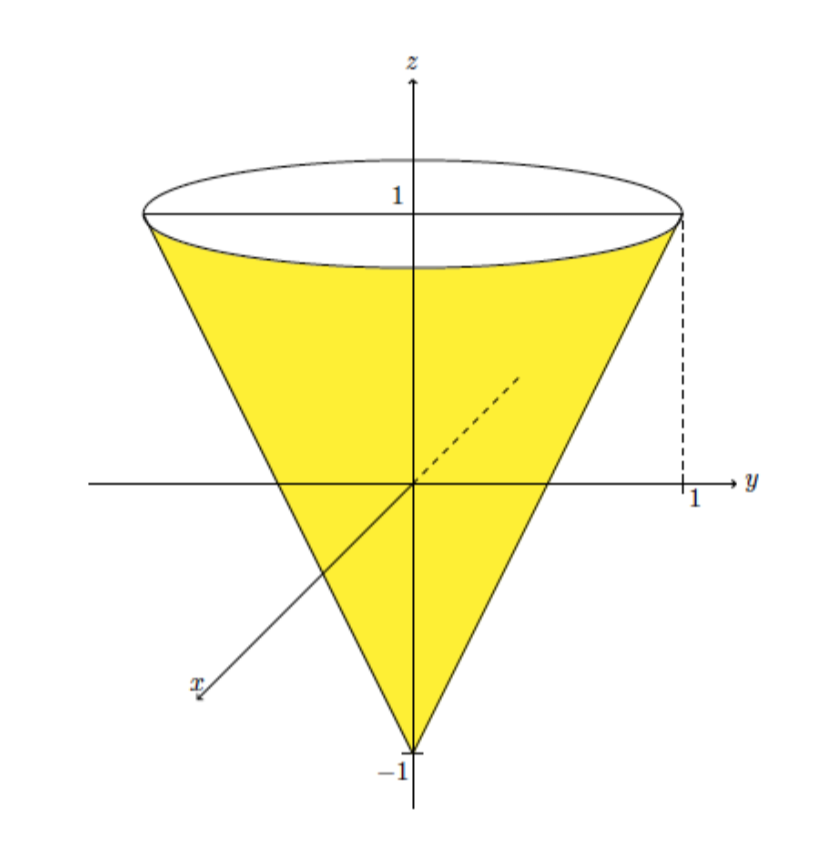
\includegraphics[width=\linewidth,keepaspectratio=true]{images/fluss}
\end{minipage}
%
\begin{minipage}[c]{0.5\textwidth}
\begin{equation*}
\begin{split}
	\text{gegeben:}\quad & \vec{F}(x,y,z) = \begin{pmatrix}
		\frac{x^2}{2} \\ -xy \\ x^2 + 3z^2 - 3
	\end{pmatrix} \\
	\text{gesucht:}\quad & \text{Fluss durch die Mantelfl{\"a}che des Kegels} \\
	& \text{(von Innen nach Aussen)} \\
	\textbf{Vorgehen:}\quad & \text{Fluss durch den ganzen Kegel} \\
	& \text{mit \textbf{Satz von Gauss} berechnen} \\
	& \text{Fluss durch Deckel} \\
	& \text{mit \textbf{Standardmethode} berechnen}
\end{split}
\end{equation*}
\end{minipage}

\clearpage

\subsection{Standardmethode}

\begin{equation*}
	\textbf{Grundsatz:}\quad\int_{\partial V} \vec{v}\cdot\vec{n}\ do
\end{equation*}

\begin{equation*}
\begin{split}
	\text{Normalvektor:}\quad & \vec{n} = \begin{pmatrix}
		0 \\ 0 \\ 1
	\end{pmatrix} \\
	\text{Vektorfeld anpassen:}\quad & z = 1 \Rightarrow \vec{F} = \begin{pmatrix}
		\frac{x^2}{2} \\ -xy \\ x^2
	\end{pmatrix} \\
	\textbf{Grundsatz anwenden:}\quad & \iint_D \begin{pmatrix}
		0 \\ 0 \\ 1
	\end{pmatrix}\begin{pmatrix}
		\frac{x^2}{2} \\ -xy \\ x^2
	\end{pmatrix} dxdy = \iint_D x^2\ dxdy \\
	\textbf{Koordinatentransformation:}\quad & \int_0^{2\pi} \int_0^1 r^3\cos^2(\phi)\ drd\phi = \frac{\pi}{4}
\end{split}
\end{equation*}

\subsection{Satz von Gauss}

\begin{equation*}
	\textbf{Grundsatz:}\quad\int_{\partial V} \vec{v}\cdot\vec{n}\ do = \int_V \text{div}(\vec{v})\ d\mu
\end{equation*}
wobei $\vec{n}$ die nach aussen gerichtete Normale l{\"a}ngs $\partial V$ bezeichnet.

\begin{equation*}
\begin{split}
	\text{Divergenz berechnen:}\quad & \text{div}(\vec{F}) = 6z \\
	\textbf{Grundsatz anwenden:}\quad & \int_{-1}^1 dz \int_0^{2\pi} d\phi \int_0^{\frac{z+1}{2}} 6zr\ dr = 2\pi
\end{split}
\end{equation*}

\emph{Bemerkung:} In diesem Beispiel wurden zylindrische Koordinaten benutzt.

\subsection{Satz von Stokes}

\paragraph{Anforderung:} Einfacher in $\mathbb{R}^3$, der Rand muss im positiven mathematischen Sinn umlaufen werden (d.h. im Gegenuhrzeigersinn)

\begin{equation*}
	\textbf{Grundsatz:}\quad\int_{\gamma = \partial C} \vec{v} \cdot d\vec{s} = \int_C \text{rot}(\vec{v}) \cdot \vec{n}\ do
\end{equation*}

\clearpage

\section{Kurvendiskussion}

\begin{table}[H]
\centering
\begin{tabular}{|c|c|c|}
\hline
Extremalstelle & $f'(x) =  0 \land f''(x) \neq 0$ \\ \hline
Minimalstelle & $f'(x) = 0 \land f''(x) > 0$ \\ \hline
Maximalstelle & $f'(x) = 0 \land f''(x) < 0$ \\ \hline
Wendepunkt & $f''(x) = 0 \land f'''(x) \neq 0$ \\ \hline
Sattelpunkt & $f'(x) = 0 \land f''(x) = 0 \land f'''(x) \neq 0$ \\ \hline
\end{tabular}
\end{table}

\begin{description}[labelindent=16pt,style=multiline,leftmargin=6cm, noitemsep]
	\item[kritischer Punkt:] $p_0 \in \Omega$ f{\"u}r welchen $\text{rank}(df(p_0)) < \min\{m,n\}$ gilt
	\item[Kandidaten f{\"u}r Extrema:] $p_0 \in \Omega$ f{\"u}r welchen $df(p_0) = 0$ gilt
\end{description}

\subsection{Extremwertaufgaben ohne Nebenbedingungen}

\begin{enumerate}[noitemsep]
	\item Kandidaten f{\"u}r Extrema finden $df(x)=0$
	\item Bestimmung:
	\begin{enumerate}[noitemsep]
		\item $\text{Hess}(f)(p_0)$ positiv definit $\Rightarrow$ lokales Minimum
		\item $\text{Hess}(f)(p_0)$ negativ definit $\Rightarrow$ lokales Maximum
		\item $\text{Hess}(f)(p_0)$ indefinit $\Rightarrow$ Sattelpunkt
	\end{enumerate}
\end{enumerate}

\emph{Bemerkung:} Falls alle Eigenwerte von $A$ gr{\"o}sser als $0$ sind, dann ist $A$ \textbf{positiv definit}. Hat $A$ sowohl positive als auch negative Eigenwerte, so ist sie \textbf{indefinit}.

\subsection{Extremwertaufgaben mit Nebenbedingungen}

\paragraph{Beweis}\mbox{}\\

Falls es sich um eine stetige Funktion auf einem kompakten Gebiet handelt, so nimmt $f$ gem{\"a}ss Weierstrass ein Supremum und Infimum an. Daraus folgt, dass $f$ auf dem Gebiet ein Maximum und Minimum besitzt.

\paragraph{1. Kandidaten im Innern des Gebiets:}

\begin{enumerate}[noitemsep, label=\roman*]
	\item $df(x,y) = 0$ aufl{\"o}sen
	\item {\"U}berpr{\"u}fen, ob gefundene Punkte wirklich im Gebiet sind
\end{enumerate}

\paragraph{2. Kandidaten auf den Randst{\"u}cken des Gebiets:}

\begin{enumerate}[noitemsep, label=\roman*]
	\item $df(x,y) - \lambda dg(x,y) - \mu dh(x,y) = 0$ aufl{\"o}sen
	\item {\"U}berpr{\"u}fen, ob gefundene Punkte wirklich auf dem Rand sind
	\item $dg(x,y) = 0$ aufl{\"o}sen und {\"u}berpr{\"u}fen, ob gefunden Punkte Nebenbedingung erf{\"u}llen
	\item Eckpunkte des Randst{\"u}ckes {\"u}berpr{\"u}fen
\end{enumerate}

$\Rightarrow$ Benutze ein System hergeleitet von $df(x,y) - \lambda dg(x,y) - \mu dh(x,y) = 0$ und den verschiedenen Nebenbedingungen. \\ 

\emph{Tipp:} Ist das Randst{\"u}ck nicht differenzierbar, muss man es in mehrere Teilstrecken aufteilen. \\

\end{document}
